
In the proposed architecture, the SmartBox plays the role of acquiring the data that is transmitted wirelessly by the Biostickers.
Each SmartBox is associated to a single patient, captures the data of each Biosticker associated with that patient and stores it in a local database for redundancy. 
It should also be capable of analyzing and process the data in real time, before propagating it to the higher layers in the system architecture, in order to reduce computation and networking overhead on the Smart Gateway. The \acs{WoW} project also foresees the usage of a classification algorithm in the SmartBox to determine the body pose of the patient, as well as filtering the respiration data to account for signal fluctuations caused by sudden movements by the patient.  

\section{Deciding on a Hardware Platform}

In the context of the dissertation, two different \acl{SBC}s (\acs{SBC}) were considered for the development of the SmartBox: a Raspberry Pi 4 Model B and an UDOO BOLT v3. In the following sections we will discuss and compare the characteristics of each platform. 

\subsubsection{Raspberry Pi 4 Model B}

Raspberry Pi denotes a series of \acs{SBC}s which are developed by the Raspberry Pi Foundation, a UK-based charity that aims to educate the general public about the power of computing and digital making, in association with Broadcom. It is one of the most popular hardware platforms used by developers due to its accessible price and community support.
At the time of the writing of this dissertation, the Raspberry Pi 4 Model B is the latest revision of the Raspberry Pi series, powered by Broadcom BCM2711 System on a Chip (SoC).

\begin{figure}[H]
    \centering
    \includegraphics[width=0.45\linewidth]{images/raspberrypi-image.jpg}
    \caption{Raspberry Pi 4 Model B.}
    \label{fig:raspberrypi-image}
\end{figure}

\subsubsection{UDOO BOLT V3}

As stated by the manufacturer\footnote{Product Website: https://www.udoo.org/discover-the-udoo-bolt/}, the ``UDOO BOLT is a quantum leap compared to current maker boards''. It represents a series of high performance \acs{SBC}, equipped with the latest generation of AMD Ryzen Embedded SoC. Additionally, it contains an Arduino Compatible microcontroller (connected via UART), making it the UDOO BOLT extremely versatile with its.
The UDOO Bolt is incredibly well supported by UDOO. And since it runs desktop Linux distros and Windows 10, third-party support is top-notch. Unfortunately, it doesn't have nearly the same community support of Raspberry Pi.

The UDOO BOLT V3 is the entry-level product of the series, but it is still capable of outperforming full-fledged computers such as the Apple MacBook 13", which just goes to show how powerful these \acs{SBC}s can be.

\begin{figure}[H]
    \centering
    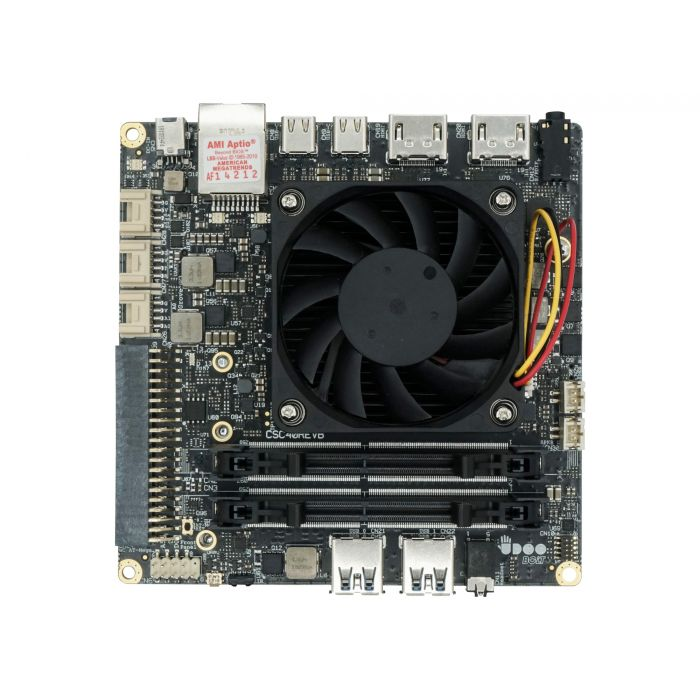
\includegraphics[width=0.45\linewidth]{images/udoobolt-image.jpg}
    \caption{Udoo Bolt V3.}
    \label{fig:udoobolt-image}
\end{figure}

\subsection{Comparing the Hardware Platforms}

In order to decide on which platform to pick for the development of the project, it's crucial to compare the specification of both boards, which can be seen in the Table \ref{tab:comparsion-hardwareplatform}.

\renewcommand{\arraystretch}{2}
\begin{table}[H]
    \centering
    \begin{tabular}{r|l|l}
        %\textbf{Features} 
        & \textbf{Raspberry Pi 4B}& \textbf{UDOO BOLT V3}  \\ \hline
        \textbf{SoC} &  \makecell{Broadcom BCM2711 (ARM v8 \\ 64-bit) 4-core @ 1.5GHz} & \makecell{AMD Ryzen™ Embedded V1202B (x86-64) \\ 2-core @ 2.3GHz (up to 3.2GHz turbo)}\\
        \textbf{RAM} & 2, 4 or 8 GB LPDDR4 & Up to 32GB DDR4 (Not included) \\ 
        \textbf{Storage} & \makecell{No internal storage, \\ SDXC Card Support} & \makecell{32GB internal eMMC + \\1x SATA III and 2x M.2 connectors}\\
        \textbf{Networking} & \makecell{2.4/5.0 GHz WiFi, Gigabit \\ Ethernet, Bluetooth 5.0, BLE} & \makecell{Gigabit Ethernet + M.2 Key E slot \\ for optional WiFi+BT module}\\ 
        \textbf{I/O Ports} & \makecell{ 2 × USB 3.0, 2 × USB 2.0, \\ 2x (Mini) HDMI} & \makecell{2x USB 3.0 Type-A, 2x USB Type-C (w/ \\ Display Port + Power Delivery), 2x HDMI} \\
        \makecell[r]{\textbf{Other} \\\textbf{Features}} & Power over Ethernet (PoE)–enabled & \makecell{Includes ATmega32U4 microcontroller\\ (Arduino Leonardo compatible), \\ RTC Battery} \\   
        \textbf{Dimensions} & 0.85 x 0.56 x 0.17 cm & 12 x 12 x 7 cm \\
        \textbf{Price} & \makecell{75.93 € (including 32GB SDXC Card\\ and case)} & \makecell{534.48 € (including external power supply\\ and 16GB RAM module)} \\
    \end{tabular}
    \caption{Specifications of the Raspberry Pi 4B and UDOO BOLT V3.}
    \label{tab:comparsion-hardwareplatform}
\end{table}
\renewcommand{\arraystretch}{1}


\paragraph{} From the Table \ref{tab:comparsion-hardwareplatform}, we immediately conclude that the Raspberry Pi is a much more affordable alternative. At over 1/7 of the price, it already has a working WiFi+BT networking module (which is not included in the UDOO BOLT), nearly identical Input/Output (I/O) port capability and a smaller size. UDOO BOLT V3 on the other hand, has a much better SoC, which should result in a much better overall computing performance.


\paragraph{} In order to understand how these differences in the specification between these two platforms translate to real-world performance, a test suite was developed and conducted. The tools developed for each test can be found here\footnote{https://github.com/WoW-Institute-of-Systems-and-Robotics/smartbox\_benchmark\_tests}. 

\paragraph{}In the next sections, we detail how each test works and discuss how each \acs{SBC} performed. 

%\subsubsection{Test 1: \textit{7-Zip} CPU Benchmark}
%\dots

\subsubsection{Test 1: Python Benchmark}

Given the data processing requirements for the SmartBox, and as Python will be used as the main scripting language for most of the SmartBox development, we developed a simple test to estimate the Python performance, or more specifically performance of arithmetic tasks, on each \acs{SBC}. On this test, each \acs{SBC} calculates the \textit{n}-th number in the Fibonacci sequence\footnote{https://en.wikipedia.org/wiki/Fibonacci\_number}, and we measure the time taken. This process is repeated 100 times for different numbers to determine the average run time for different amounts.

\begin{figure}[H]
    \centering
    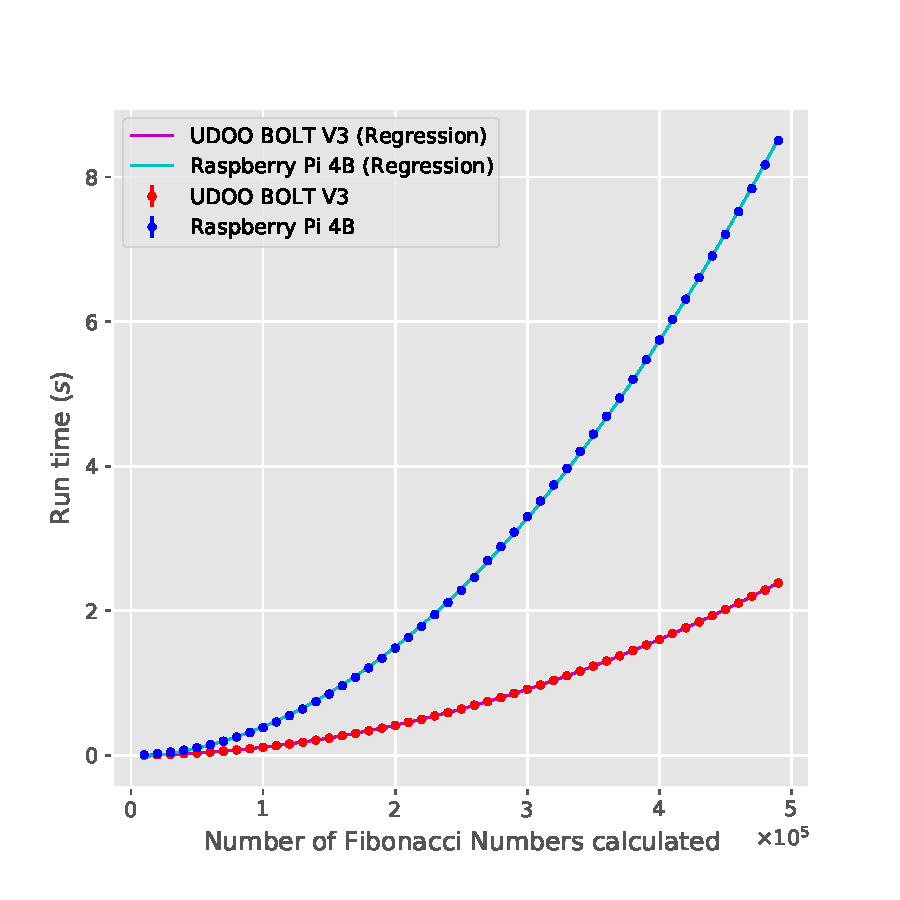
\includegraphics[width=0.6 \linewidth]{images/fibonacci-test.pdf}
    \caption [Results of the custom Python benchmark for the Raspberry Pi 4B and UDOO BOLT V3.]{ Results of the custom Python benchmark for the Raspberry Pi 4B and UDOO BOLT V3. }
    \label{fig:fibonacci-tests}
\end{figure}

From the Figure \ref{fig:fibonacci-tests}, we can observe that the time taken for computing each number increases exponentially for each platform. By analyzing the data, we can see that the UDOO BOLT V3 outperforms Raspberry Pi 4B on average by a factor of 2.7 $\pm$ 0.6.

\subsubsection{Test 2: Phoronix Test Suite}

The Phoronix Test Suite\footnote{Phoronix Test Suite - Linux Testing \& Benchmarking Platform, Automated Testing, Open-Source Benchmarking: \textit{https://www.phoronix-test-suite.com/}} is an open-source benchmarking platform used for comparing the performance of different systems. The framework provides compilations of tests for a variety of tools and is also fully customizable and expandable, allowing users to develop and automate their own tests in a clean, reproducible and easy-to-use fashion.  

For the purposes of evaluating which single board computer should be used, we chose the Python PyPerformance and PyBench, and 7-Zip test profiles provided by Phoronix\footnote{OpenBenchmarking.org - Cross-Platform, Open-Source Automated Benchmarking Platform: \textit{https://openbenchmarking.org/}}. These test profiles work by measuring the time \acs{SBC}s take to perform different tasks (\textit{e.g.} calculating the first 100 Fibonacci numbers) and calculate a quantitive score based on these run times, which is useful for comparing CPU (and more particularly Python) performance between different systems.

\todo[inline]{Todo: Add the missing Phoronix benchmark graph?}


\subsubsection{Test 3: \acs{MQTT} Benchmark}

As the SmartBox will communicate with the Smart Gateway through \acs{MQTT}, we decided to evaluate how each system handles the load associated with an \acs{MQTT} client. For this test, each \acs{SBC} ran a simple \acs{MQTT} client which was subscribing to a single topic and publishing to another topic using a given transmission rate, with an \acs{MQTT} broker in the local network.

\begin{figure}[H]
    \centering
    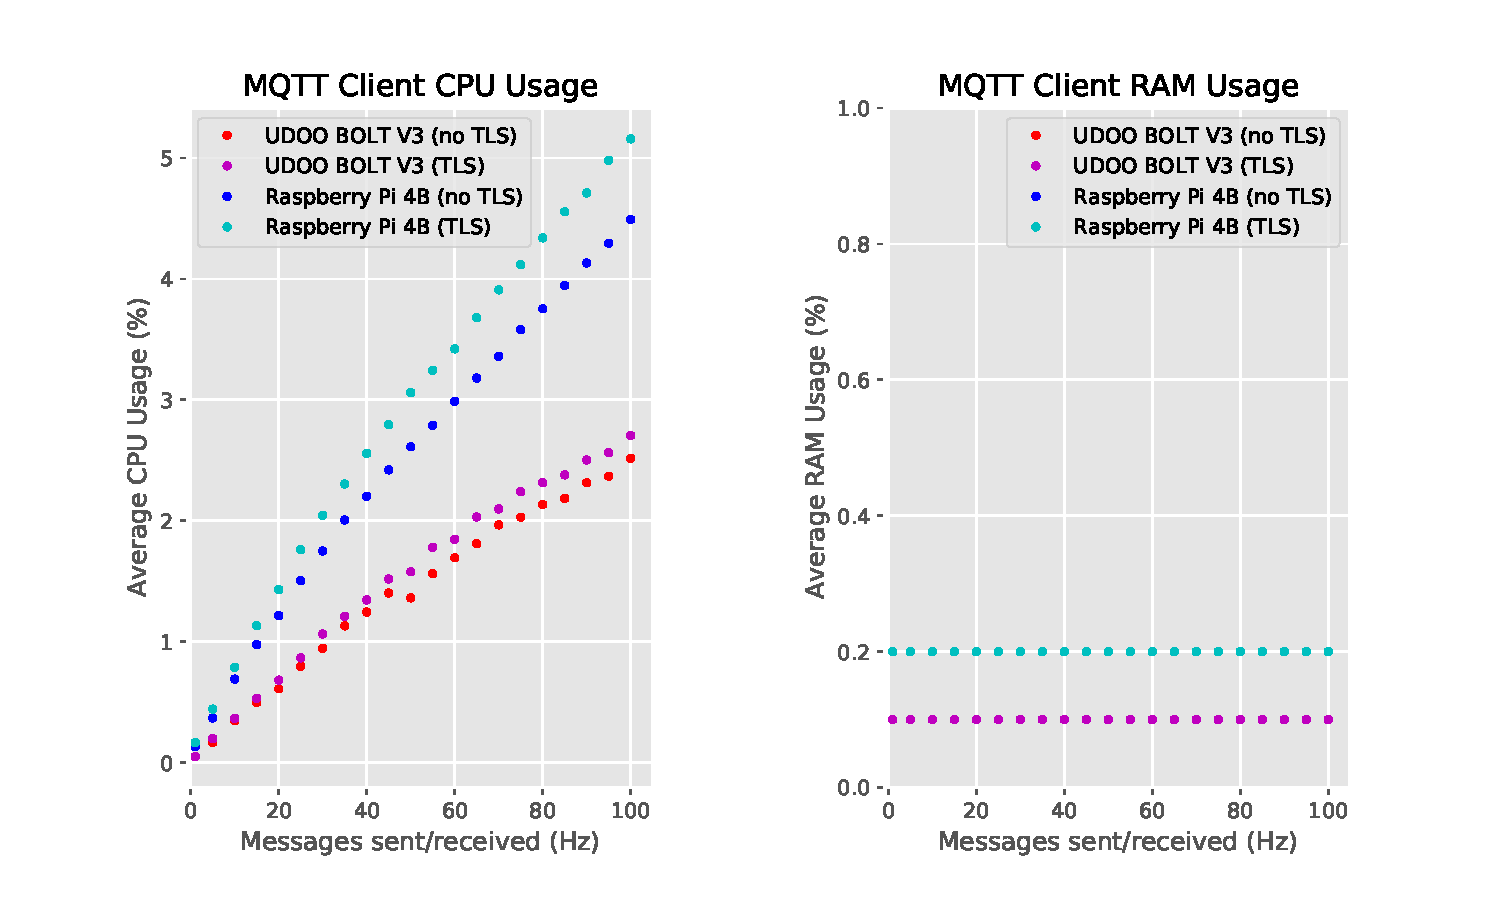
\includegraphics[width=\linewidth]{images/mqtt_test_results.pdf}
    \caption[Results of the \acs{MQTT} benchmark for Raspberry Pi 4B and UDOO BOLT V3.]{Results of the \acs{MQTT} benchmark for Raspberry Pi 4B and UDOO BOLT V3. As the transmission frequency increases, we observe that the Raspberry Pi consumes more resources than the UDOO BOLT V3, nonetheless, these are very negligible performance differences, with an impact of < 0.5\% resource usage.}
    \label{fig:mqtt-tests}
\end{figure}

The \acs{MQTT} client is a very lightweight process, and as seen in Figure \ref{fig:mqtt-tests}, is capable of running on both platforms with trivial performance impact.

\subsubsection{Conclusion}

Based on the results of our tests we conclude that UDOO BOLT V3 heavily outperforms the Raspberry Pi 4 Model B in CPU benchmarks, but shows a negligible difference in memory usage. However, we find that these performance gains do not meaningfully impact the SmartBox functionality, for example, in the \acs{MQTT} communication. Due to the extremely affordable price of the Raspberry Pi 4B, we have decided to move forward with the Raspberry Pi 4B for the development of the project.

\section{Communication with the Biostickers}

\subsection{Overview of \acf{BLE}}

\begin{figure}[H]
    \centering
    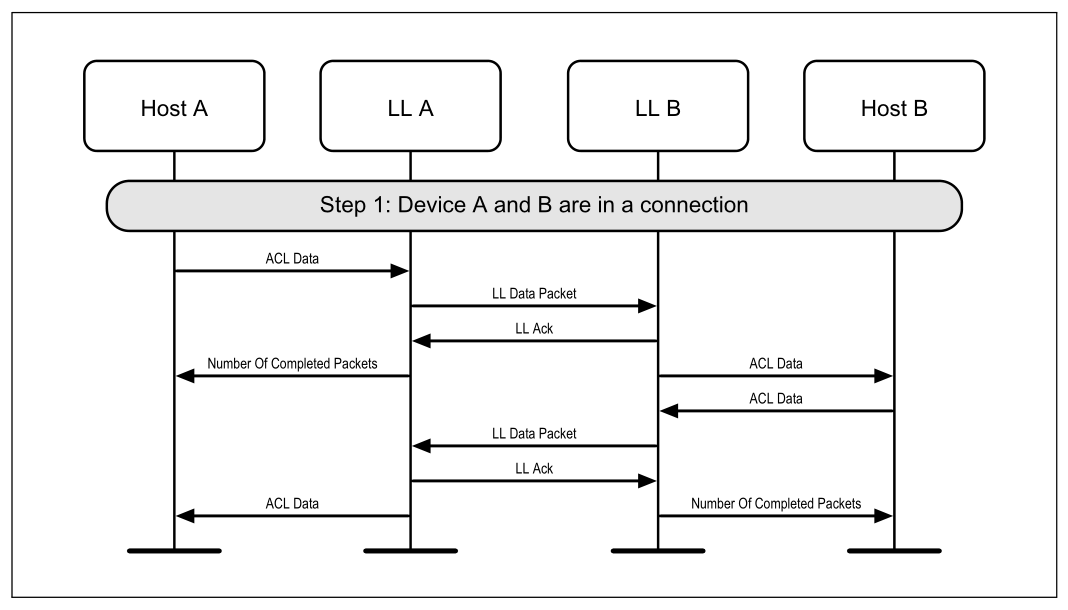
\includegraphics[width=\linewidth]{images/ble-sending-data.PNG}
    \caption[Message sequence chart between two \acs{BLE} devices sending data and replying to the request.]{Message sequence chart between two \acs{BLE} devices sending data and replying to the request. Source: \cite{Specification1999}}
    \label{fig:differences-between-cloud-services}
\end{figure}


\begin{enumerate}
    \item Slave Latency:
    \item Connection Interval:
    \item Supervisor Timeout
    \item \acs{MTU} for the \acs{ATT} protocol: 
\end{enumerate}

\subsubsection{Test 1: Roundtrip Time Measurement}

\begin{figure}[H]
    \begin{minipage}[r]{0.49\linewidth}
    \centering
    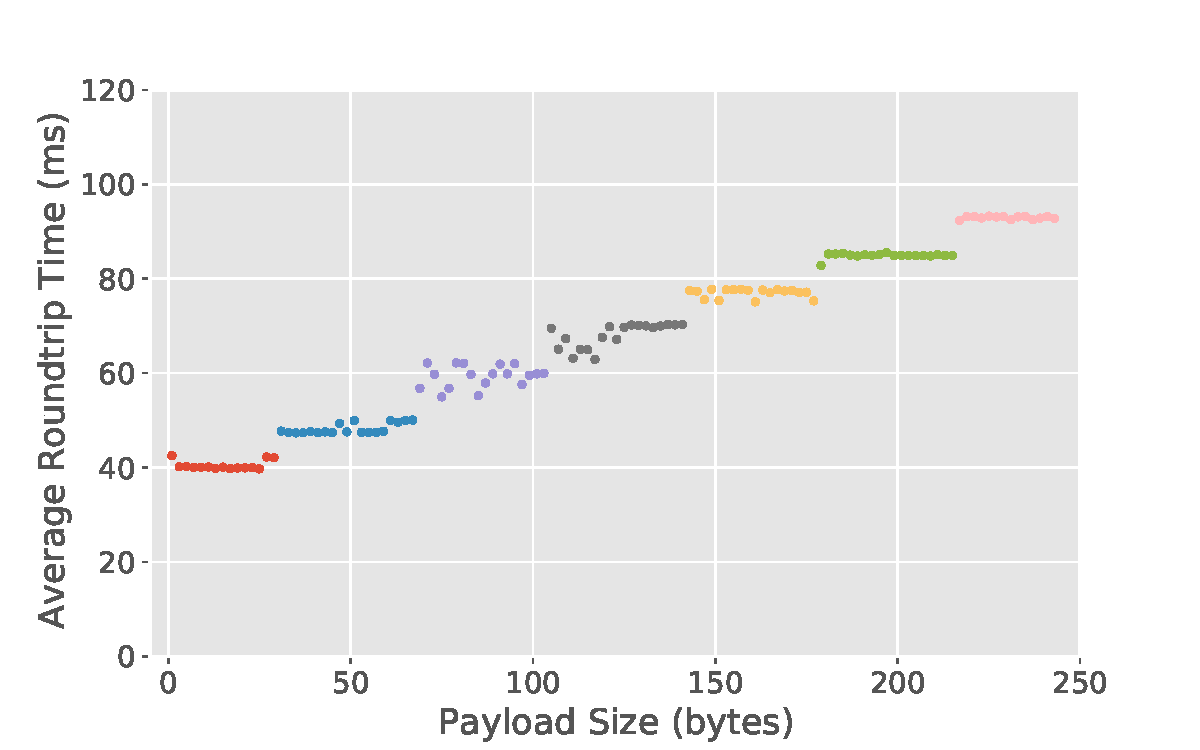
\includegraphics[width=\linewidth]{images/ble-roundtrip-hci0-0cm.pdf}
    \caption[Average \acs{BLE} connection roundtrip time at a distance of 0m.]{Average \acs{BLE} connection roundtrip time at a distance of $0\text{m} \pm 0.2$.}
    \label{fig:ble-roundtrip-6cm}
    \end{minipage}
    \begin{minipage}[l]{0.49\linewidth}
        \centering
        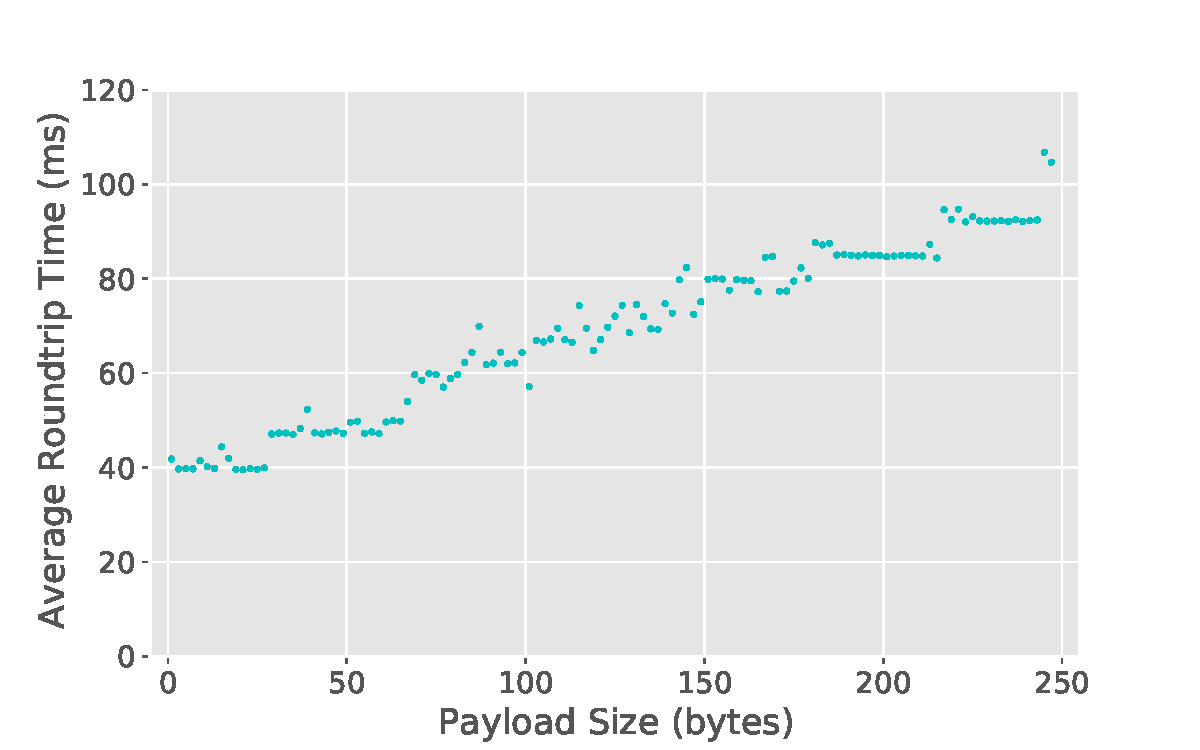
\includegraphics[width=\linewidth]{images/ble-roundtrip-hci0-300cm.pdf}
        \caption[Average \acs{BLE} connection roundtrip time at a distance of 3m.]{Average \acs{BLE} connection roundtrip time at a distance of $3\text{m} \pm 0.2$.}
        \label{fig:ble-roundtrip-9cm}
        \end{minipage}
\end{figure}


\begin{figure}[H]
    \begin{minipage}[r]{0.49\linewidth}
    \centering
    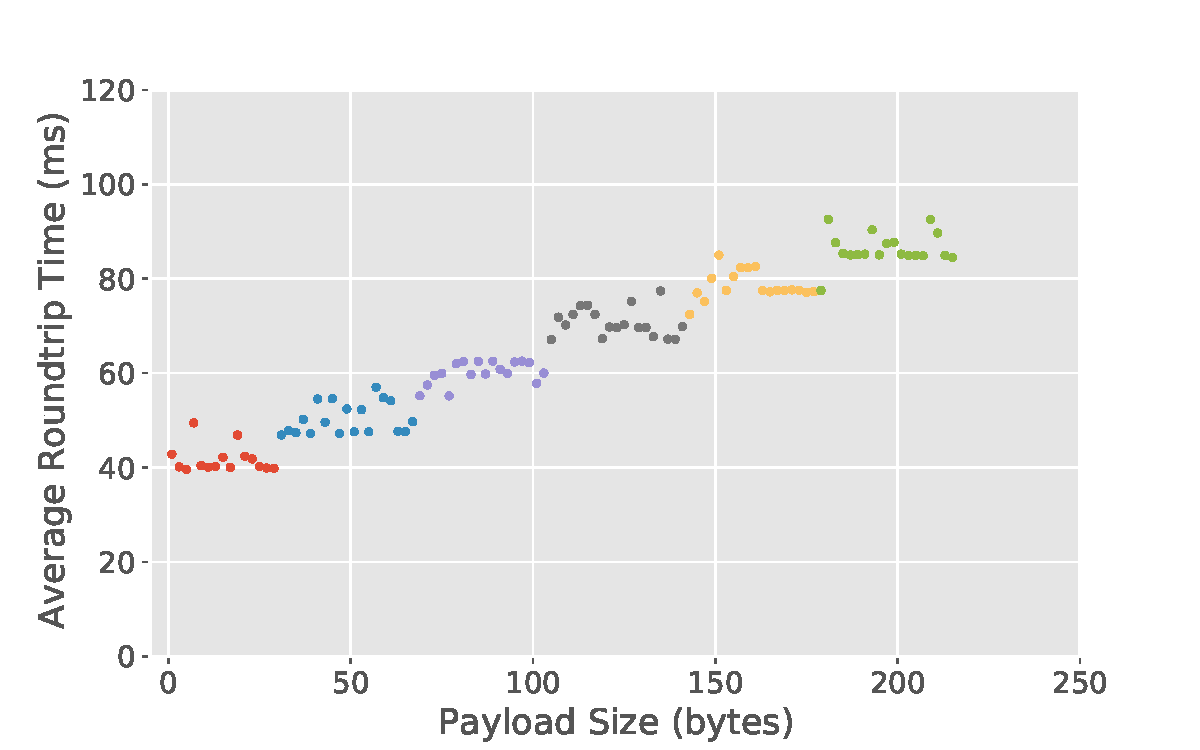
\includegraphics[width=\linewidth]{images/ble-roundtrip-hci0-600cm.pdf}
    \caption[Average \acs{BLE} connection roundtrip time at a distance of 6m.]{Average \acs{BLE} connection roundtrip time at a distance of $6\text{m} \pm 0.2$.}
    \label{fig:ble-roundtrip-6cm}
    \end{minipage}
    \begin{minipage}[l]{0.49\linewidth}
        \centering
        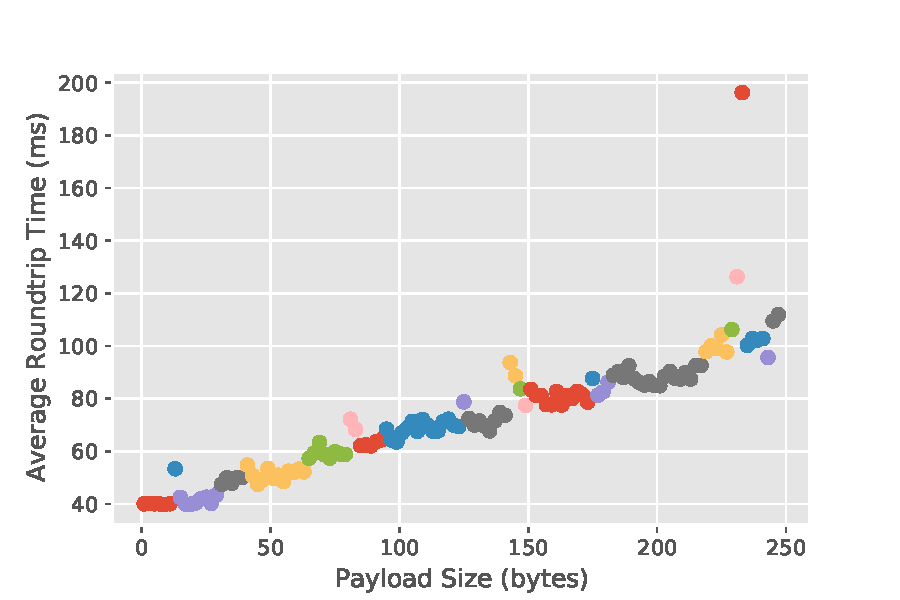
\includegraphics[width=\linewidth]{images/ble-roundtrip-hci0-900cm.pdf}
        \caption[Average roundtrip time obtained at a distance of 9m using \acs{BLE} connection.]{Average \acs{BLE} connection roundtrip time at a distance of $9\text{m} \pm 0.2$.}
        \label{fig:ble-roundtrip-9cm}
        \end{minipage}
\end{figure}

\subsubsection{Test 2: Bandwidth Measurement}


\section{Summary}
In this chapter, we \dots